% Chapter 3, Section 1: Probability Distributions

\section{Probability Distributions}
\label{sec:probability-distributions}

\subsection{Intuition: What is Probability?}

Imagine you're playing a game of dice. Before rolling, you know that each face (1 through 6) has an equal chance of appearing. This "chance" is what we call \textbf{probability} - a number between 0 and 1 that quantifies how likely an event is to occur.

In machine learning, we face uncertainty everywhere:
\begin{itemize}
    \item \textbf{Data uncertainty}: Will the next customer click on an ad?
    \item \textbf{Model uncertainty}: How confident is our neural network in its prediction?
    \item \textbf{Parameter uncertainty}: What's the best value for our model's weights?
\end{itemize}

Probability distributions are mathematical tools that help us model and work with this uncertainty systematically.

\subsection{Visualizing Probability}

Consider a simple example: predicting whether it will rain tomorrow. We might say there's a 30\% chance of rain. This means:
\begin{itemize}
    \item If we could repeat tomorrow 100 times, rain would occur about 30 times
    \item The probability of rain is 0.3
    \item The probability of no rain is 0.7
\end{itemize}

\begin{figure}[h]
\centering
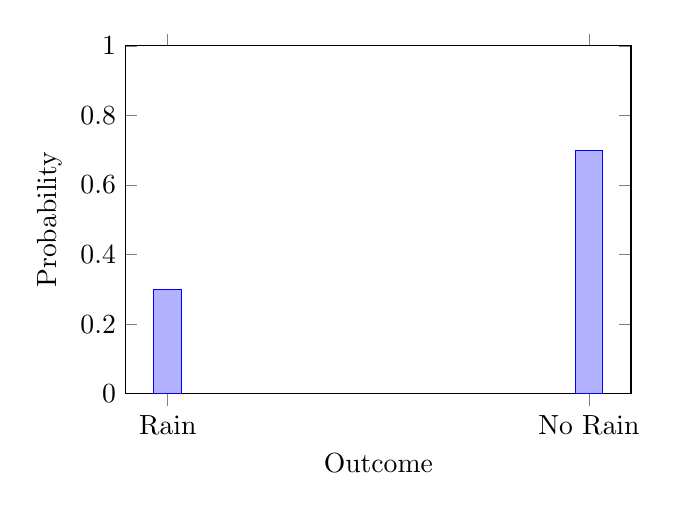
\begin{tikzpicture}
\begin{axis}[
    ybar,
    ylabel={Probability},
    xlabel={Outcome},
    xtick={1,2},
    xticklabels={Rain, No Rain},
    ymin=0,
    ymax=1,
    width=8cm,
    height=6cm
]
\addplot coordinates {(1,0.3) (2,0.7)};
\end{axis}
\end{tikzpicture}
\caption{Probability distribution for rain prediction}
\label{fig:rain-probability}
\end{figure}

Probability theory provides a mathematical framework for quantifying uncertainty. In deep learning, we use probability distributions to model uncertainty in data, model parameters, and predictions.

\subsection{Discrete Probability Distributions}

\subsubsection{Intuition: Counting Outcomes}

Think of discrete probability as counting specific outcomes. For example:
\begin{itemize}
    \item \textbf{Coin flip}: Heads (1) or Tails (0) - only 2 possible outcomes
    \item \textbf{Dice roll}: 1, 2, 3, 4, 5, or 6 - exactly 6 possible outcomes
    \item \textbf{Email classification}: Spam (1) or Not Spam (0) - binary outcome
\end{itemize}

A discrete random variable $X$ takes values from a countable set. The \textbf{probability mass function} (PMF) $P(X=x)$ assigns probabilities to each possible value:

\begin{equation}
P(X=x) \geq 0 \quad \text{for all } x
\end{equation}

\begin{equation}
\sum_{x} P(X=x) = 1
\end{equation}

\subsubsection{Example: Fair Coin}

For a fair coin, we have:
\begin{align}
P(X=0) &= 0.5 \quad \text{(Tails)} \\
P(X=1) &= 0.5 \quad \text{(Heads)}
\end{align}

\begin{figure}[h]
\centering
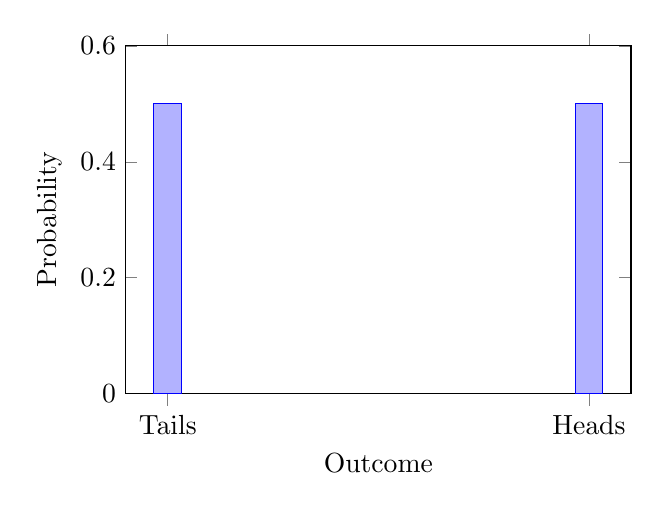
\begin{tikzpicture}
\begin{axis}[
    ybar,
    ylabel={Probability},
    xlabel={Outcome},
    xtick={0,1},
    xticklabels={Tails, Heads},
    ymin=0,
    ymax=0.6,
    width=8cm,
    height=6cm
]
\addplot coordinates {(0,0.5) (1,0.5)};
\end{axis}
\end{tikzpicture}
\caption{Probability mass function for a fair coin}
\label{fig:coin-pmf}
\end{figure}

\subsection{Continuous Probability Distributions}

\subsubsection{Intuition: Measuring Instead of Counting}

Unlike discrete variables, continuous variables can take any value within a range. Think of:
\begin{itemize}
    \item \textbf{Height of people}: Can be 5.7 feet, 5.73 feet, 5.732 feet, etc.
    \item \textbf{Temperature}: Can be 72.3°F, 72.34°F, 72.341°F, etc.
    \item \textbf{Neural network weights}: Can be 0.1234, 0.12345, 0.123456, etc.
\end{itemize}

Since there are infinitely many possible values, we can't assign probabilities to individual points. Instead, we use \textbf{density} - how "concentrated" the probability is in different regions.

A continuous random variable can take any value in a continuous range. We describe it using a \textbf{probability density function} (PDF) $p(x)$:

\begin{equation}
p(x) \geq 0 \quad \text{for all } x
\end{equation}

\begin{equation}
\int_{-\infty}^{\infty} p(x) \, dx = 1
\end{equation}

The probability that $X$ falls in an interval $[a, b]$ is:

\begin{equation}
P(a \leq X \leq b) = \int_a^b p(x) \, dx
\end{equation}

\subsubsection{Example: Normal Distribution}

The most common continuous distribution is the \textbf{normal (Gaussian) distribution}, which looks like a bell curve:

\begin{figure}[h]
\centering
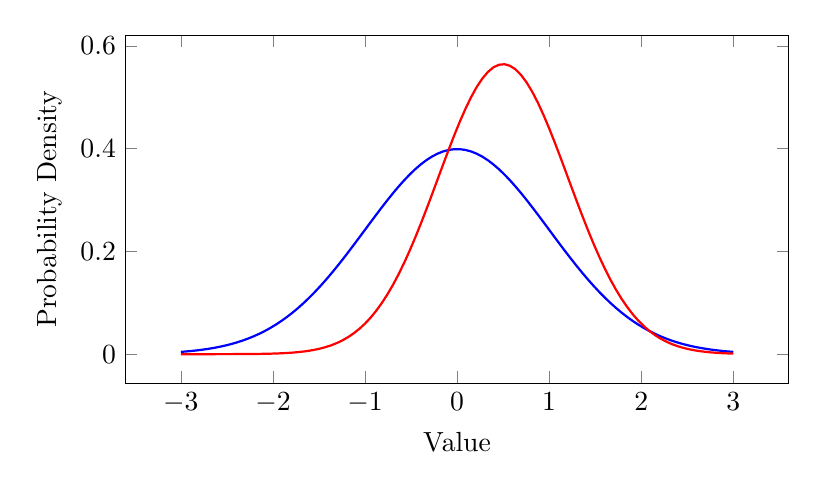
\begin{tikzpicture}
\begin{axis}[
    ylabel={Probability Density},
    xlabel={Value},
    domain=-3:3,
    width=10cm,
    height=6cm,
    samples=100
]
\addplot[blue, thick] {1/sqrt(2*pi) * exp(-x^2/2)};
\addplot[red, thick] {1/sqrt(2*pi*0.5) * exp(-(x-0.5)^2/(2*0.5))};
\end{axis}
\end{tikzpicture}
\caption{Two normal distributions with different means and standard deviations}
\label{fig:normal-distributions}
\end{figure}

The area under the curve between any two points gives the probability of the variable falling in that range.

\subsection{Joint and Marginal Distributions}

\subsubsection{Intuition: Multiple Variables Together}

In real-world scenarios, we often deal with multiple variables simultaneously:
\begin{itemize}
    \item \textbf{Weather prediction}: Temperature AND humidity
    \item \textbf{Image classification}: Pixel values at different positions
    \item \textbf{Stock prices}: Multiple stocks in a portfolio
\end{itemize}

The \textbf{joint distribution} tells us about the probability of combinations of values, while \textbf{marginal distributions} tell us about individual variables when we ignore the others.

\subsubsection{Example: Weather Data}

Consider a simple weather dataset with two variables:
\begin{itemize}
    \item $X$: Temperature (Hot/Cold)
    \item $Y$: Humidity (High/Low)
\end{itemize}

\begin{table}[h]
\centering
\begin{tabular}{|c|c|c|c|}
\hline
 & $Y=$ High & $Y=$ Low & \textbf{Marginal} \\
\hline
$X=$ Hot & 0.3 & 0.2 & \textbf{0.5} \\
$X=$ Cold & 0.1 & 0.4 & \textbf{0.5} \\
\hline
\textbf{Marginal} & \textbf{0.4} & \textbf{0.6} & \textbf{1.0} \\
\hline
\end{tabular}
\caption{Joint probability table for weather data}
\label{tab:weather-joint}
\end{table}

For multiple random variables $X$ and $Y$, the \textbf{joint distribution} $P(X, Y)$ describes their combined behavior. The \textbf{marginal distribution} is obtained by summing (or integrating) over the other variable:

\begin{equation}
P(X=x) = \sum_{y} P(X=x, Y=y)
\end{equation}

For continuous variables:

\begin{equation}
p(x) = \int p(x, y) \, dy
\end{equation}

From our weather example:
\begin{itemize}
    \item $P(X=\text{Hot}) = 0.3 + 0.2 = 0.5$ (marginal probability of hot weather)
    \item $P(Y=\text{High}) = 0.3 + 0.1 = 0.4$ (marginal probability of high humidity)
\end{itemize}
